\section{The Bigger Picture}

% ---------------------------------------------------------------- Some perspectives (transition)
\begin{frame}{Some perspectives to close on\dots}
\vfill
\begin{itemize}
    \setlength{\itemsep}{1.0em}
    \item Reinforcement Learning as an \textbf{Engineering Tool}
    \item Reinforcement Learning and the \textbf{Real World}
    \item Reinforcement Learning as ``\textbf{Universal}'' Learning
\end{itemize}
\vfill
\begin{center}\footnotesize\itshape
Less about algorithms now --- more about what RL is \emph{for}.
\end{center}
\end{frame}

% ---------------------------------------------------------------- Engineering tool (compressed 5->1)
\begin{frame}{RL as an engineering tool}
\begin{columns}[c]
\begin{column}{0.58\textwidth}
\begin{itemize}\footnotesize\itemsep0.5em
    \item Seen from engineering, RL is barely new. Classical control already says:
          \emph{characterize} the system, \emph{simulate} it, then \emph{control} it.
    \item RL just swaps the last step: characterize, simulate, \textbf{run RL}.
    \item Its real role is a \empr{powerful inversion engine} --- given a simulator and a
          goal, it searches out the actions that achieve it.
    \item \empy{Slogan:} \textbf{anything you can simulate, you can control.}
    \item \empy{Main weakness:} you \emph{still need to simulate} --- and the real world
          is hard to simulate.
\end{itemize}
\end{column}
\begin{column}{0.42\textwidth}
\centering
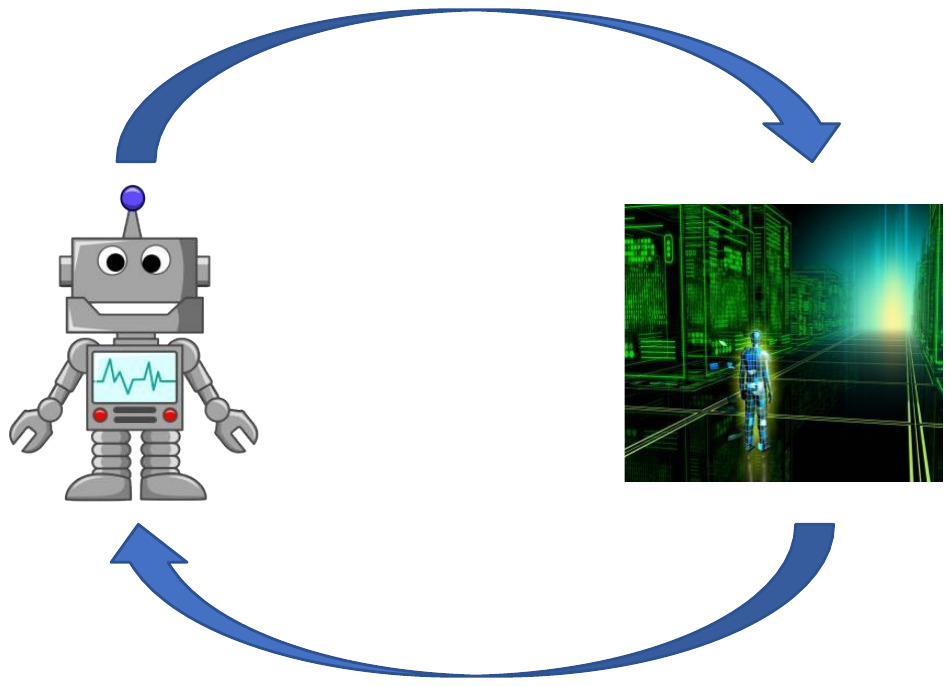
\includegraphics[width=\linewidth]{images/meta-rl-open/figures/simulate-control.jpg}
\end{column}
\end{columns}
\end{frame}

% ---------------------------------------------------------------- Moravec (keep S47)
\begin{frame}{Moravec's paradox}
\footnotesize Moravec's paradox seems like a statement about AI, but it is really a
statement about the \emph{physical universe}.\normalsize
\vspace{0.3em}
\begin{columns}[c]
\begin{column}{0.36\textwidth}
\centering
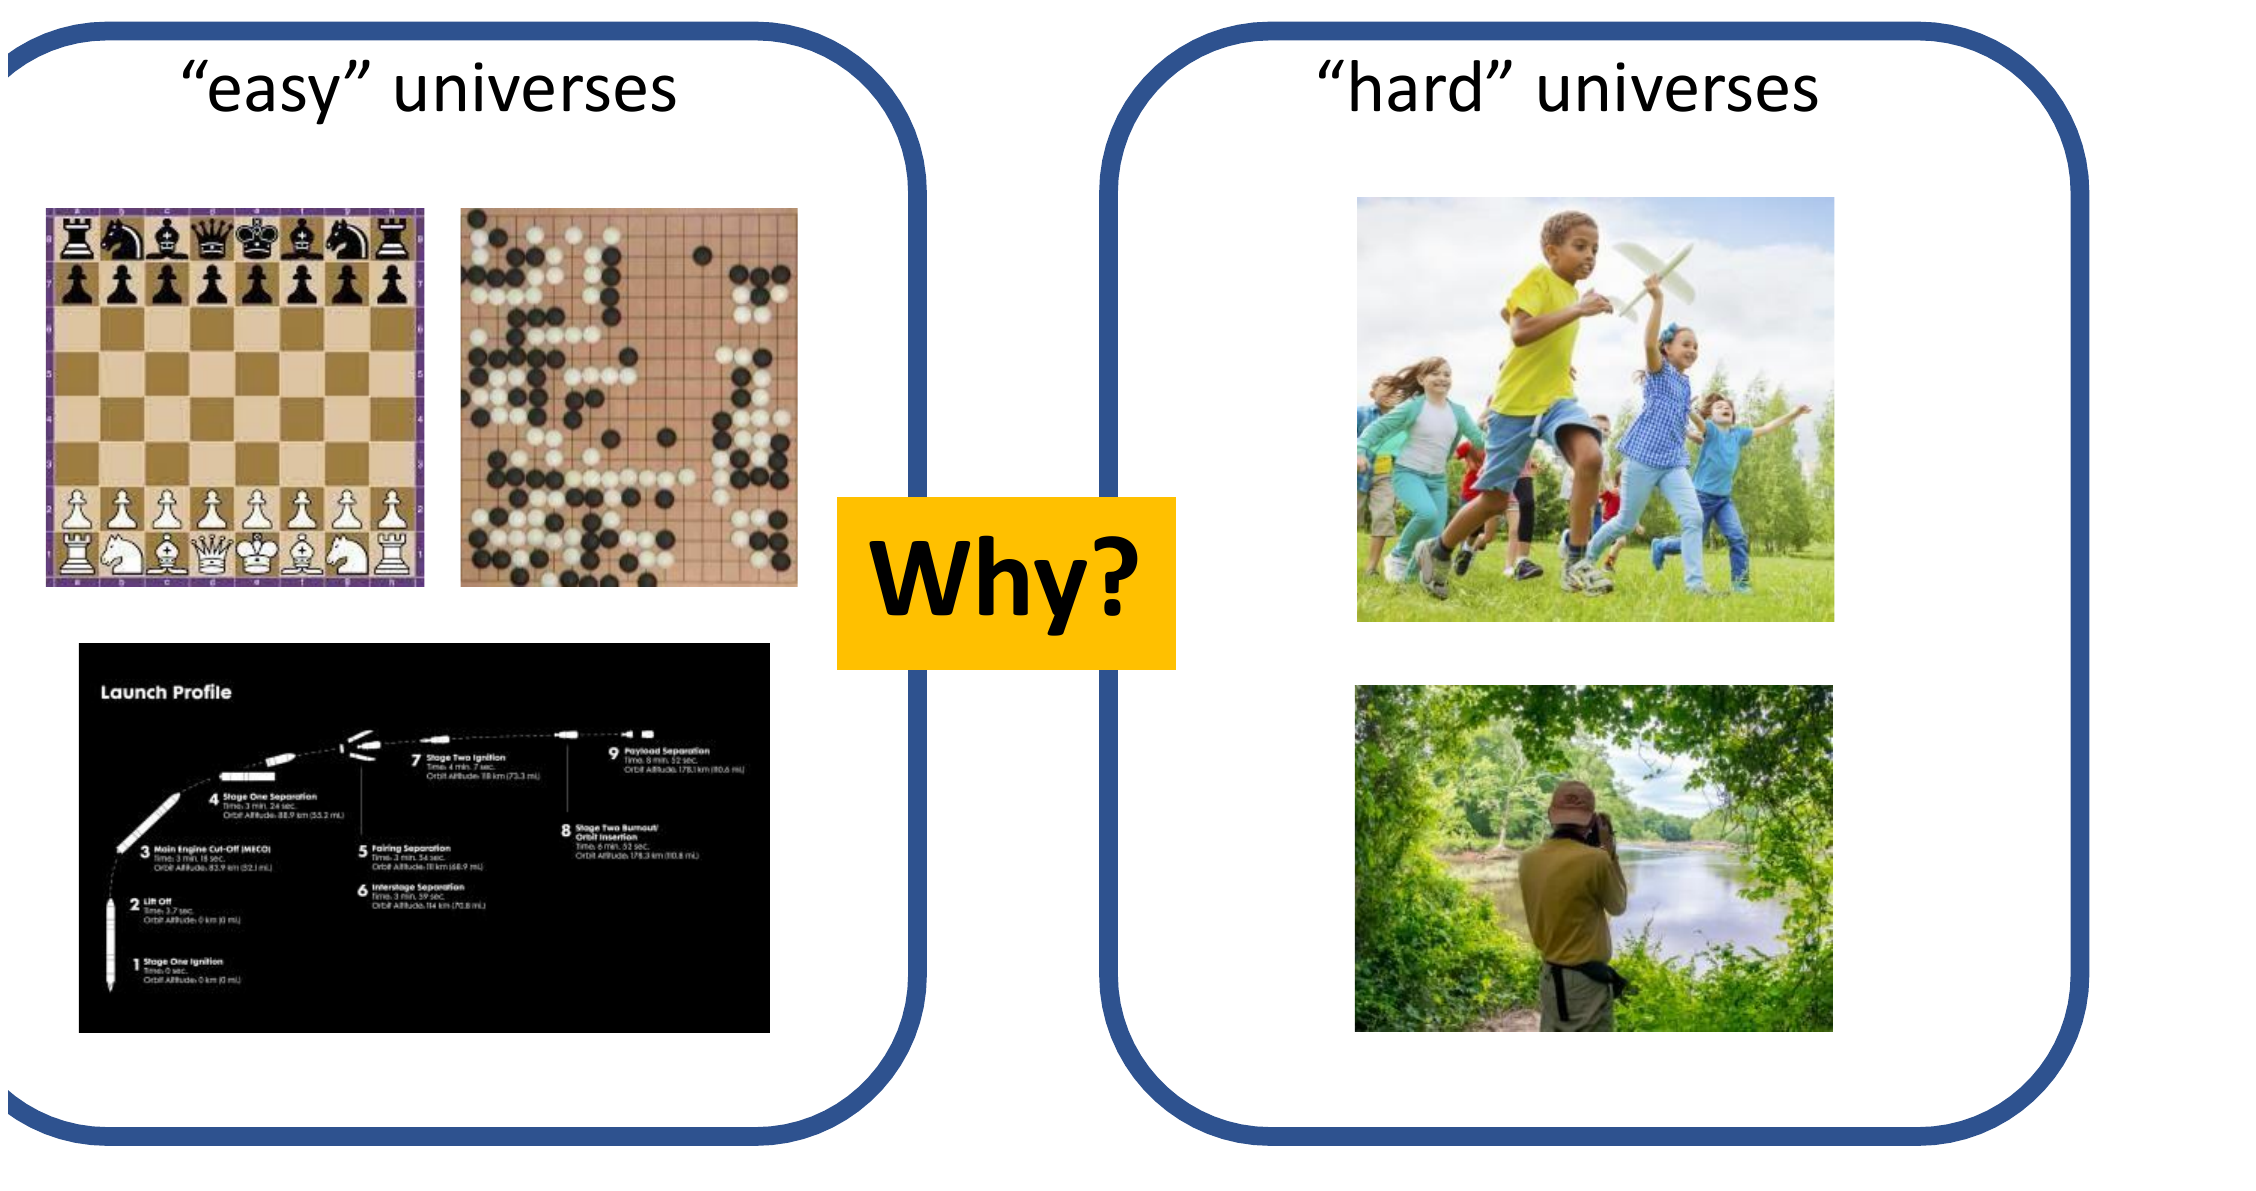
\includegraphics[width=\linewidth]{images/meta-rl-open/figures/moravec-univ.jpg}
\end{column}
\begin{column}{0.64\textwidth}
\footnotesize
``We are all prodigious olympians in perceptual and motor areas, so good that we make
the difficult look easy. Abstract thought, though, is a new trick, perhaps less than 100
thousand years old. We have not yet mastered it. It is not all that intrinsically
difficult; it just seems so when we do it.'' \hfill --- Hans Moravec
\vspace{0.7em}

``The main lesson of thirty-five years of AI research is that the hard problems are easy
and the easy problems are hard. The mental abilities of a four-year-old that we take for
granted --- recognizing a face, lifting a pencil, walking across a room, answering a
question --- in fact solve some of the hardest engineering problems ever conceived.''
\hfill --- Steven Pinker
\end{column}
\end{columns}
\end{frame}

% ---------------------------------------------------------------- Island / survival (keep S48)
\begin{frame}{What does this have to do with RL?}
\begin{columns}[c]
\begin{column}{0.34\textwidth}
\centering
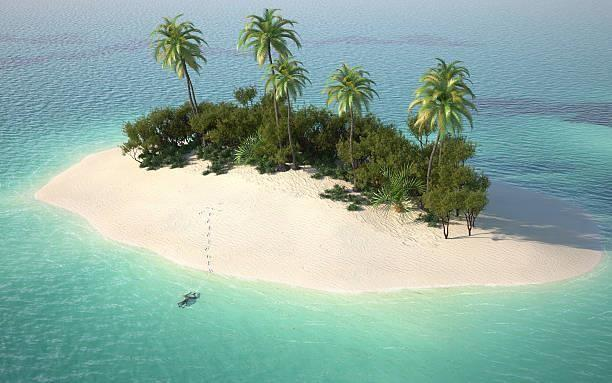
\includegraphics[width=\linewidth]{images/meta-rl-open/figures/island.jpg}
\end{column}
\begin{column}{0.66\textwidth}
\centering How do we engineer a system that can deal with the unexpected?
\vspace{0.6em}
\begin{itemize}
    \item Minimal external supervision about what to do
    \item Unexpected situations that require adaptation
    \item Must discover solutions autonomously
    \item Must ``stay alive'' long enough to discover them!
\end{itemize}
\end{column}
\end{columns}
\vfill
\begin{itemize}
    \item Humans are extremely good at this
    \item Current AI systems are extremely bad at this
    \item RL in principle can do this, and nothing else can
\end{itemize}
\end{frame}

% ---------------------------------------------------------------- Easy vs hard universes (keep S49)
\begin{frame}{So what's the problem?}
\begin{center}\footnotesize
RL in principle can do this, and nothing else can --- \emph{but we rarely study this kind
of setting in RL research!}
\end{center}
\vfill
\renewcommand{\arraystretch}{1.25}
\centering\footnotesize
\begin{tabular}{p{0.42\textwidth} p{0.42\textwidth}}
\textbf{``easy'' universes} & \textbf{``hard'' universes}\\
\hline
success $=$ high reward (``optimal control'') & success $=$ ``survival'' (``good enough control'')\\
closed world, rules are known & open world, everything must come from data\\
lots of simulation & no simulation (because rules are unknown)\\
Main question: can RL algorithms optimize really well & Main question: can RL generalize and adapt\\
\end{tabular}
\vfill
{\footnotesize RL should be really good in the ``hard'' universes!}
\end{frame}

% ---------------------------------------------------------------- What's the point / emergent (keep S55)
\begin{frame}{This all seems really hard, what's the point?}
\begin{columns}[c]
\begin{column}{0.32\textwidth}
\centering
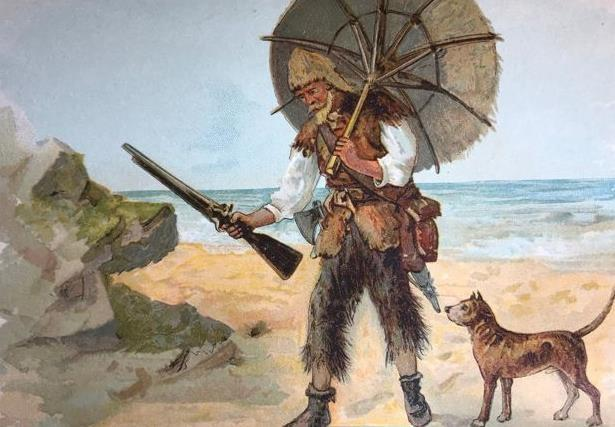
\includegraphics[width=\linewidth]{images/meta-rl-open/figures/crusoe.jpg}
\end{column}
\begin{column}{0.68\textwidth}
\begin{center}Why is this interesting?\end{center}
\vspace{0.3em}
\begin{itemize}
    \item It's exciting to see what solutions intelligent agents come up with
    \item Most exciting if they come up with something we don't expect
    \item This requires the world they inhabit to admit novel solutions
    \item This means that world must be complicated enough!
\end{itemize}
\end{column}
\end{columns}
\vfill
{\footnotesize To see interesting emergent behavior, we must train our systems in
environments that actually require interesting emergent behavior!}
\end{frame}

% ---------------------------------------------------------------- Open-endedness (NEW - pays off Day 9)
\begin{frame}{Open-endedness: no fixed task distribution at all}
\begin{columns}[c]
\begin{column}{0.56\textwidth}
\begin{itemize}\footnotesize\itemsep0.5em
    \item If complexity must \emph{come from the environment}, where does an endless
          supply of it come from?
    \item \textbf{Self-play (Day 9)} was one engine: agents generate their own
          \empr{curriculum} automatically, each one's progress raising the bar for the
          others.
    \item \textbf{Open-endedness / POET:} \emph{co-evolve} the tasks \emph{and} the agents
          --- never a fixed objective, always a new frontier just beyond reach.
    \item The endpoint of today's thread: meta and multi-task still assumed
          $\mathcal{M}_i \sim p(\mathcal{M})$; open-endedness gives up even that ---
          \empy{no fixed task distribution at all.}
\end{itemize}
\end{column}
\begin{column}{0.44\textwidth}
\centering
\resizebox{0.95\linewidth}{!}{%
\begin{tikzpicture}[font=\scriptsize, ar/.style={-{Stealth[length=1.6mm]}}]
  \node[draw, rounded corners, fill=boxtan!55, minimum width=2.2cm] (tasks) {tasks};
  \node[draw, rounded corners, fill=mlgreen!50, right=2.2cm of tasks, minimum width=2.2cm] (agents) {agents};
  \draw[ar, thick] (tasks) to[bend left=30] node[above,font=\tiny]{harder tasks} (agents);
  \draw[ar, thick] (agents) to[bend left=30] node[below,font=\tiny]{stronger agents} (tasks);
  \node[below=0.9cm of $(tasks)!0.5!(agents)$, align=center, font=\scriptsize]
        {co-evolution:\\ complexity never saturates};
\end{tikzpicture}}
\end{column}
\end{columns}
\srcnote{\tiny Wang, Lehman, Clune, Stanley. Paired Open-Ended Trailblazer (POET). 2019.}
\end{frame}

% ---------------------------------------------------------------- Wolpert postulate (keep S59)
\begin{frame}{Stepping back: why do we need learning at all?}
\begin{columns}[c]
\begin{column}{0.56\textwidth}
\footnotesize
Why do we need \textbf{machine learning} anyway?
\vspace{0.4em}

{\setlength{\fboxsep}{4pt}%
\fcolorbox{red}{white}{\begin{minipage}{0.95\linewidth}
\textbf{A postulate:} We need machine learning for one reason and one reason only ---
that's to produce \textbf{\underline{adaptable and complex decisions}}.
\end{minipage}}}
\vspace{0.5em}

\raisebox{-0.45\height}{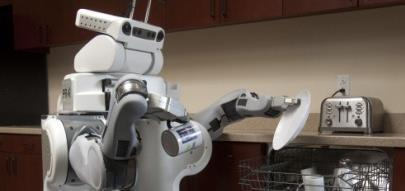
\includegraphics[height=0.85cm]{images/meta-rl-open/figures/ml-robot.jpg}}\;\;
Decision: how do I move my joints?\par\vspace{0.3em}
\raisebox{-0.45\height}{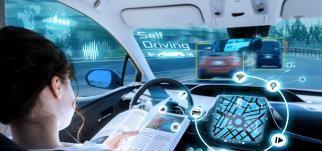
\includegraphics[height=0.85cm]{images/meta-rl-open/figures/ml-car.jpg}}\;\;
Decision: how do I steer the car?\par\vspace{0.3em}
\raisebox{-0.45\height}{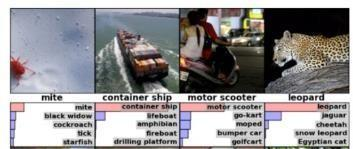
\includegraphics[height=0.85cm]{images/meta-rl-open/figures/ml-imagenet.jpg}}\;\;
What is the decision? The image label? {\color{red}\textbf{Usually not!}}\par\vspace{0.3em}
What happens with that label afterwards? \emph{These are {\color{red}\textbf{decisions}} ---
they lead to {\color{red}\textbf{consequences}}}
\end{column}
\begin{column}{0.42\textwidth}
\footnotesize
\textbf{Aside:} why do we need \textbf{brains} anyway?

\vspace{0.4em}
\colorbox{blue!6}{%
\begin{minipage}{0.94\linewidth}
\centering
\begin{minipage}{0.34\linewidth}\centering
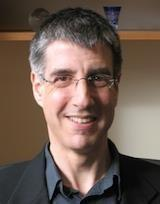
\includegraphics[width=\linewidth]{images/meta-rl-open/figures/wolpert-photo.jpg}\\[0.2em]
{\scriptsize\textbf{Daniel Wolpert}}\\
{\tiny (knows quite a lot about brains)}
\end{minipage}\hfill
\begin{minipage}{0.32\linewidth}\centering

\includegraphics[width=\linewidth]{images/meta-rl-open/figures/brain-icon.jpg}
\end{minipage}

\vspace{0.5em}
{\scriptsize\itshape ``We have a brain for one reason and one reason only --- that's to
produce \textbf{adaptable and complex movements}. Movement is the only way we have
affecting the world around us\dots I believe that to understand movement is to understand
the whole brain.''}
\end{minipage}}
\end{column}
\end{columns}
\end{frame}

% ---------------------------------------------------------------- Universal learning: cheap data (compress S57-58)
\begin{frame}{RL as ``universal'' learning: using cheap data}
\begin{columns}[c]
\begin{column}{0.56\textwidth}
\begin{itemize}\footnotesize\itemsep0.5em
    \item The lesson of large-scale ML: progress comes from \textbf{diverse data} and
          \emph{reducing the supervision burden} per example.
    \item RL's angle on this: it can learn from \empr{cheap, un-curated experience} ---
          not just hand-labelled examples.
    \item \textbf{Offline RL (Day 8):} squeeze a good policy out of a \emph{fixed dataset}
          of past interaction --- no new environment steps, no fresh labels.
    \item That reframes RL as a general recipe for turning \emph{logged experience} into
          \emph{decisions} --- the same engine, pointed at whatever data is cheap.
\end{itemize}
\end{column}
\begin{column}{0.44\textwidth}
\centering
\resizebox{0.95\linewidth}{!}{%
\begin{tikzpicture}[font=\scriptsize, ar/.style={-{Stealth[length=1.8mm]}, line width=1pt}]
  \node[draw, rounded corners, fill=boxtan!55, minimum width=2.6cm] (data) {cheap / logged data};
  \node[draw, rounded corners, fill=sysblue!45, below=8mm of data, minimum width=2.6cm] (rl) {offline RL};
  \node[draw, rounded corners, fill=mlgreen!55, below=8mm of rl, minimum width=2.6cm] (pol) {a policy (decisions)};
  \draw[ar] (data)--(rl); \draw[ar] (rl)--(pol);
\end{tikzpicture}}
\end{column}
\end{columns}
\end{frame}

% ---------------------------------------------------------------- Offline RL for LLMs (callback S64-66)
\begin{frame}{A concrete case: offline RL for LLM dialogue}
\begin{columns}[c]
\begin{column}{0.6\textwidth}
\begin{itemize}\footnotesize\itemsep0.5em
    \item \empr{Recall Day 8:} offline RL learns from a fixed dataset with no environment
          interaction (MOReL / MOPO / COMBO --- pessimism keeps it honest).
    \item Point that engine at \textbf{multi-turn dialogue}: an LLM is a cheap
          \emph{simulator of human conversation}.
    \item Instead of \emph{imitating} human replies, RL optimises for a downstream
          \textbf{outcome} (persuade, book, resolve) using the LLM's model of how people
          respond.
    \item RL $+$ LLM shines exactly when a task is \emph{easy to simulate} but
          \emph{hard to do optimally}.
\end{itemize}
\end{column}
\begin{column}{0.4\textwidth}
\centering
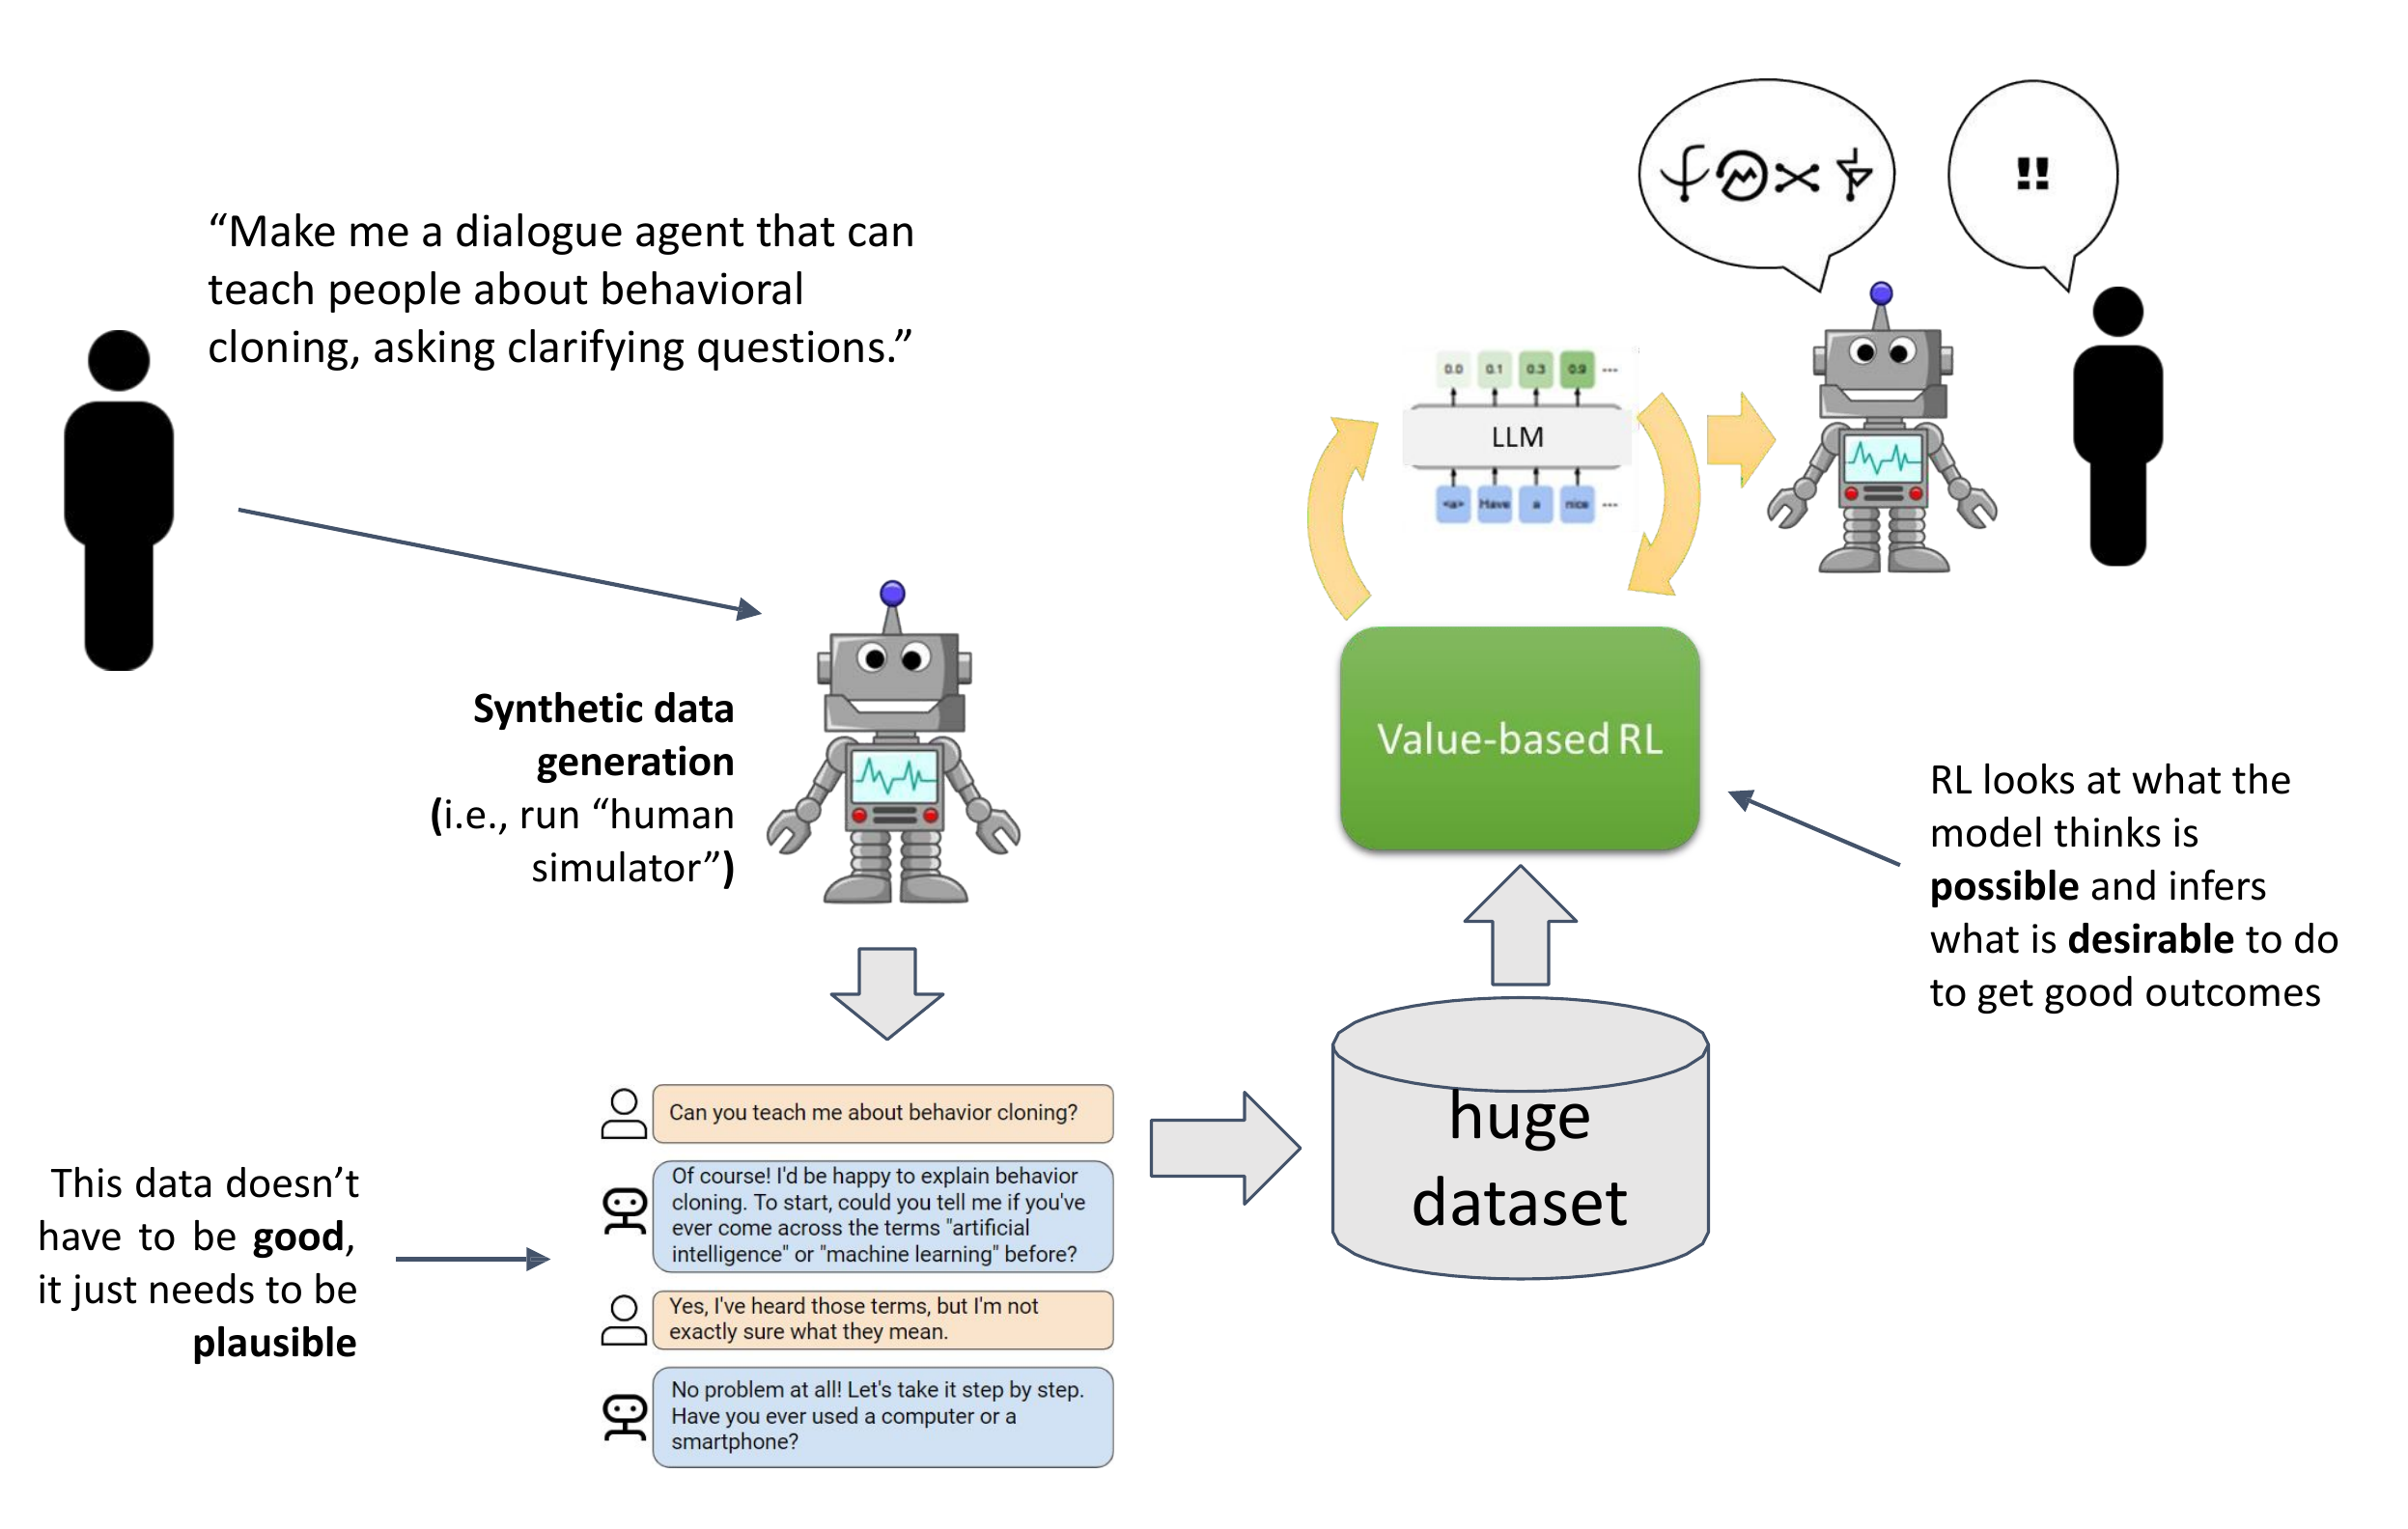
\includegraphics[width=\linewidth]{images/meta-rl-open/figures/dialogue-mb.png}
\end{column}
\end{columns}
\srcnote{\tiny Hong, Levine, Dragan. Goal-Directed Dialogue via RL on Imagined Conversations. 2023.}
\end{frame}

% ---------------------------------------------------------------- Learning as intelligence (keep S68)
\begin{frame}{Learning as the basis of intelligence}
\begin{columns}[c]
\begin{column}{0.62\textwidth}
\begin{itemize}
    \item Reinforcement learning $=$ can reason about decision making
    \item Deep models $=$ allows RL algorithms to learn and represent complex
          input-output mappings
\end{itemize}
\vspace{0.8em}
\textbf{Deep models are what allow reinforcement learning algorithms to solve complex
problems end to end!}
\end{column}
\begin{column}{0.38\textwidth}
\centering
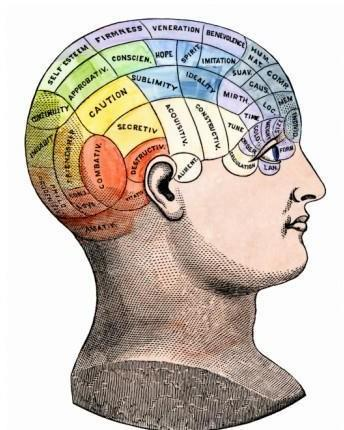
\includegraphics[width=0.8\linewidth]{images/meta-rl-open/figures/brain.jpg}
\end{column}
\end{columns}
\end{frame}

% ---------------------------------------------------------------- The cake (keep S69 as-is)
\begin{frame}{What is missing?}
\centering
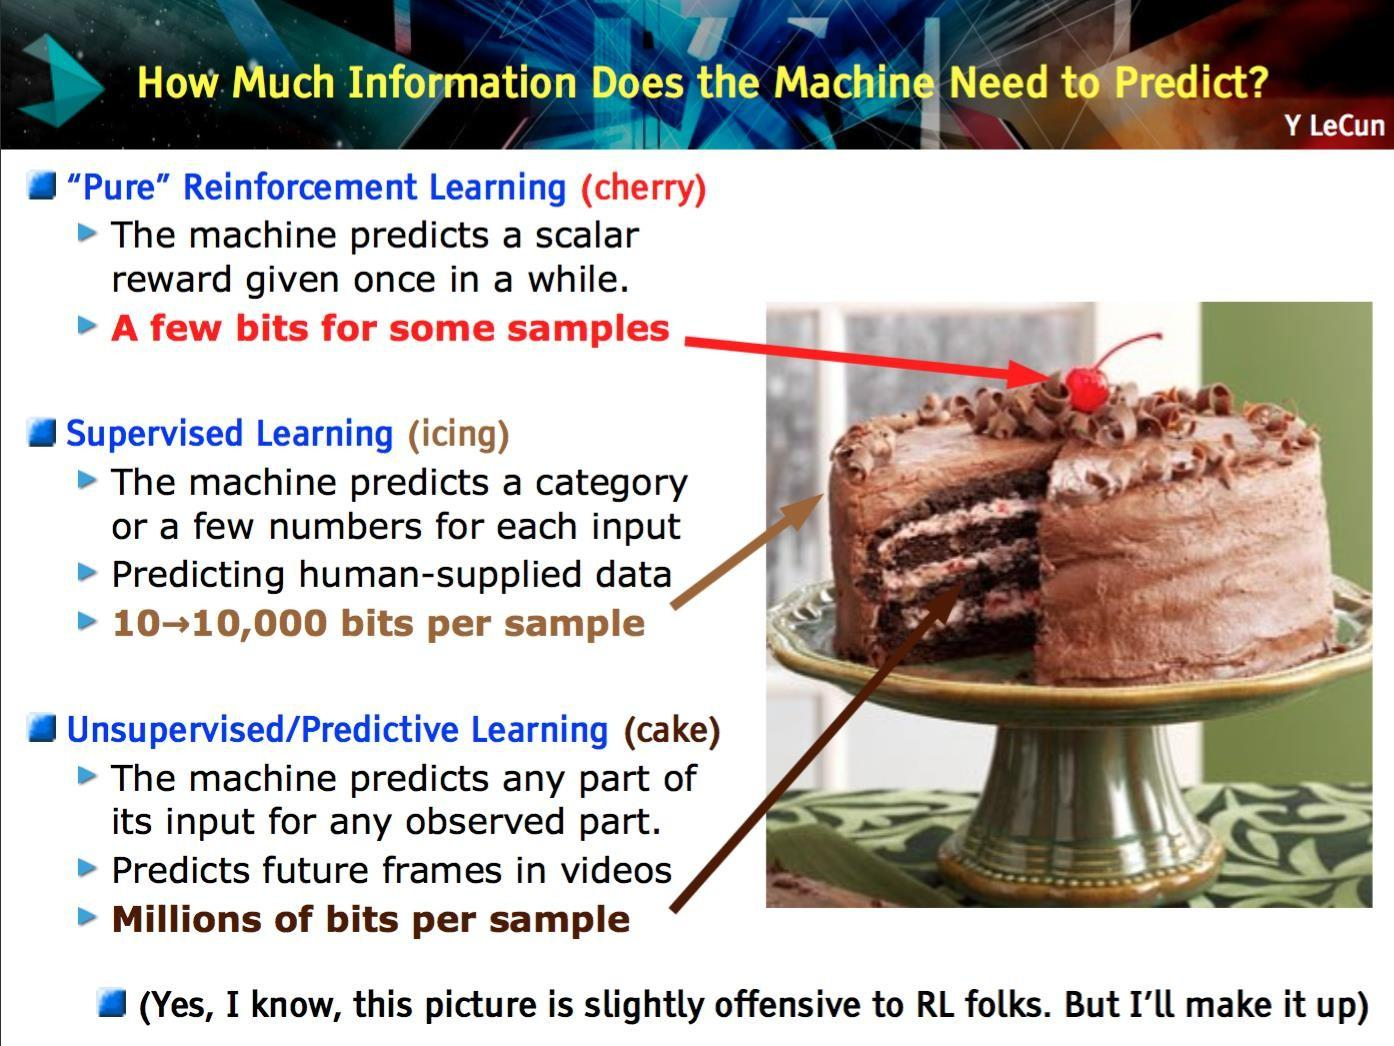
\includegraphics[width=\linewidth,height=0.82\textheight,keepaspectratio]{images/meta-rl-open/figures/whats-missing.jpg}
\end{frame}
